
%% 
%% Copyright 2007, 2008, 2009 Elsevier Ltd
%% 
%% This file is part of the 'Elsarticle Bundle'.
%% ---------------------------------------------
%% 
%% It may be distributed under the conditions of the LaTeX Project Public
%% License, either version 1.2 of this license or (at your option) any
%% later version.  The latest version of this license is in
%%    http://www.latex-project.org/lppl.txt
%% and version 1.2 or later is part of all distributions of LaTeX
%% version 1999/12/01 or later.
%% 
%% The list of all files belonging to the 'Elsarticle Bundle' is
%% given in the file `manifest.txt'.
%% 
%% Template article for Elsevier's document class `elsarticle'
%% with harvard style bibliographic references
%% SP 2008/03/01

\documentclass[preprint,12pt]{elsarticle}

%% Use the option review to obtain double line spacing
%% \documentclass[authoryear,preprint,review,12pt]{elsarticle}

%% Use the options 1p,twocolumn; 3p; 3p,twocolumn; 5p; or 5p,twocolumn
%% for a journal layout:
%% \documentclass[final,1p,times,authoryear]{elsarticle}
%% \documentclass[final,1p,times,twocolumn,authoryear]{elsarticle}
%% \documentclass[final,3p,times,authoryear]{elsarticle}
%% \documentclass[final,3p,times,twocolumn,authoryear]{elsarticle}
%% \documentclass[final,5p,times,authoryear]{elsarticle}
%% \documentclass[final,5p,times,twocolumn,authoryear]{elsarticle}

%% For including figures, graphicx.sty has been loaded in
%% elsarticle.cls. If you prefer to use the old commands
%% please give \usepackage{epsfig}

%% The amssymb package provides various useful mathematical symbols
\usepackage{amsmath,amssymb,bm}
\usepackage[dvips,colorlinks=true,citecolor=green]{hyperref}
\usepackage{verbatim}

%% The amsthm package provides extended theorem environments
%% \usepackage{amsthm}
%% The lineno packages adds line numbers. Start line numbering with
%% \begin{linenumbers}, end it with \end{linenumbers}. Or switch it on
%% for the whole article with \linenumbers.
%% \usepackage{lineno}
\journal{NDT \& E International}
\begin{document}
	\begin{frontmatter}
		%% Title, authors and addresses
		%% use the tnoteref command within \title for footnotes;
		%% use the tnotetext command for theassociated footnote;
		%% use the fnref command within \author or \address for footnotes;
		%% use the fntext command for theassociated footnote;
		%% use the corref command within \author for corresponding author footnotes;
		%% use the cortext command for theassociated footnote;
		%% use the ead command for the email address,
		%% and the form \ead[url] for the home page:
		%% \title{Title\tnoteref{label1}}
		%% \tnotetext[label1]{}
		%% \author{Name\corref{cor1}\fnref{label2}}
		%% \ead{email address}
		%% \ead[url]{home page}
		%% \fntext[label2]{}
		%% \cortext[cor1]{}
		%% \address{Address\fnref{label3}}
		%% \fntext[label3]{}
		
		\title{Parallel spectral element method for model-assisted structural health monitoring}
		
		%% use optional labels to link authors explicitly to addresses:
		%% \author[label1,label2]{}
		\address[pk]{Institute of Fluid Flow Machinery, Polish Academy of Sciences, Poland}
		\address[jm]{Goethe University, Germany}
		
		\author{Pawel Kudela\fnref{pk}}
		\author{Jochen Moll\fnref{jm}}
		
		
		\begin{abstract}
			%% Text of abstract
			A new approach for numerical simulation of the wave propagation in a composite plate is presented in this paper. Problem is realised by the 2D--3D coupled time domain spectral element method. All components used in the simulation are decomposed from each other. A connection between them is guaranteed by the interface elements realised by Lagrange multipliers. With this type of scheme, one can avoid a modelling of all the components by the three--dimensional (3D) spectral elements. In particular, the computation time can be reduced by using two-–dimensional (2D) elements for adhesive layer modelling. Otherwise, 3D elements are very inefficient because a convergence of Central Difference Time Integration Method applied for solving an equation of motion is strongly correlated with the size of the smallest element. Numerical calculations were performed for the composite plate modelled by the 3D solid elements with a piezoelectric transducer bonded to the plate by the adhesive layer modelled by 2D shell elements. The simulations were carried out for an adhesive layer of various thickness for the excitation frequency in the range 50 to 200 kHz. The presented model was verified by experimental data obtained by the laser vibrometer.
		\end{abstract}
		
		\begin{keyword}
			%% keywords here, in the form: keyword \sep keyword
			Spectral element method \sep Guided waves \sep CFRP plates \sep interface elements \sep Lagrange multipliers.
			%% PACS codes here, in the form: \PACS code \sep code
			
			%% MSC codes here, in the form: \MSC code \sep code
			%% or \MSC[2008] code \sep code (2000 is the default)
			
		\end{keyword}
		
	\end{frontmatter}
	
	%% \linenumbers
	
	%% main text
	\section{Introduction}
	\section{Flat shell spectral element}
	\section{Implementation by using Matlab Parallel Computing Toolbox}
	\section{Interpolation on uniform grid}
	\section{Experimental validation}
	\section{Exemplary applications}
	\section{Conclusions}
	\begin{comment}
	\label{Intro}
	Composite materials due to high strength--to--weight ratio are extensively used in aircraft and aerospace industry \cite{mrazova2013advanced, mangalgiri1999composite} and civil constructions \cite{pendhari2008application}. However, these complex structures are exposed to a risk of different types of failures such as delamination, cracks, disbonds, poor cure and voids. Defects can occur either during a manufacturing process, storage or in--service life \cite{jollivet2013damage}. 
	
	Due to a specificity of the failures and mechanical properties of the composites classical Non-Destructive Techniques (NDT) are unavailing thus the advanced methods for damage detections are required. The method with excellent potential for applications in NDT and Structural Health Monitoring (SHM) is a technique based on Guided Waves (GW) propagation \cite{ostachowicz2011guided}. GW are waves propagating in an elastic medium between two parallel free surfaces. Excitation and sensing of the GW can be realised by the lightweight and inexpensive piezoelectric transducers (PZT) \cite{giurgiutiumicromechatronics}. The compact PZT can be surface--bonded to the inspected structure or even embedded between the composite plies so that the measurements can be conducted in situ. The PZT transducers generate high forces with broadband frequency, so methods based on GW can detect different types and size of damage for a large inspected area \cite{su2006guided}. Moreover, certain algorithms do not require a baseline model. Among numerous techniques developed for damage detection and localisation, the most popular are pitch--catch \cite{ihn2008pitch, sikdar2017structural}, pulse--echo \cite{guo1993interaction, kudela2008damage}, phase array \cite{lu2006crack, ostachowicz2008elastic} and time--reversal mirror \cite{fink1992time, eremin2016analytically}. 
	
	Many existed numerical methods were adopted, or new methods were developed for the GW propagation analysis during the recent decades. The finite element method (FEM) applied to solve many engineering problems has also found application for modelling of wave propagation \cite{talbot1975finite, koshiba1984finite}. The incontestable advantage of this method is a possibility of modelling of structures varied in shape, size, dimension, and boundary conditions. However, due to low order approximation fine meshing is required and an error of the wave propagation increases with the time of the simulation. Other classical methods applied for modelling elastic waves propagation are the finite difference method (FDM) \cite{strikwerda1989finite} and the boundary element method (BEM) \cite{brebbia2012boundary}. 
	
	A new method for simulation of GW -- local interaction simulation approach (LISA),  was presented in \cite{delsanto1992connection}. In this method heuristic approach is implemented instead of solving a finite differential equation. On the other hand, Doyle proposed a spectral element method based on fast Fourier transformation (FFT SEM) \cite{doyle1989wave}. This technique is very efficient, but it is limited to simple one--dimensional (1D) problems. The flexibility of conventional methods was combined with the efficiency of FFT--based SEM in the formulation of time--domain Spectral Element Method (SEM) proposed by Patera \cite{patera1984spectral}. A comprehensive overview regarding numerical wave propagation analysis one can find in work presented in \cite{raghavan2007guided, willberg2015simulation}.
	
	A thickness and shear modulus of the adhesive interface layer has a significant effect on a transfer of stress and strain from the host structure to the transducer and \textit{vice versa}. According to \cite{crawley1987use}, if the shear modulus increases or thickness decreases shear lag becomes less significant, and shear is effectively transferred mainly near to the end of the PZT. Ha and Chang \cite{ha2010adhesive} presented the parametric studies of generating and recording of the Lamb waves in an isotropic plate depending on the thickness and material properties of the adhesive layer. The authors adopted a hybrid spectral element method (\textit{i.e.} a combination of SEM and Gauss quadrature with two points for formulation a mass and stiffness matrices, for validation of the experimental measurements \cite{ha2009optimizing}). Islam and Huang \cite{islam2014understanding} studied the effects of the adhesive layer on the electromechanical impedance (EMI) of the PZT sensor. The adhesive thickness for optimisation of Lamb waves in SHM was also considered in \cite{islam2016effects, willberg2013increasing}. Ashawin \textit{et al.} \cite{ashwin2014formulation} proposed SEM formulation by 2D elements coupled with Lagrange multipliers for simulation of GW propagation in an aluminium plate with analysis of the effect of the adhesive layer on the sensor response. 
	
	In this paper, a novel scheme for a simulation of propagation of GW excited by the PZT transducer adhesive bonded to a composite plate is presented. All components are decomposed similarly to FEM \cite{farhat1998two} and defined independently by two types of the elements. PZT transducer and the host plate are modelled by 3D solid elements \cite{kudela20093d}, whereas the adhesive layer is modelled by 2D elements \cite{ashwin2014formulation}.
	
	The displacements coupling between the adjacent elements is forced by Lagrange multipliers \cite{wohlmuth2000mortar,flemisch2006elasto}. This type of formulation enables reduction of computation time in comparison to full 3D modelling without losing accuracy.
	
	\section{Time--domain spectral element method formulation}
	\label{SEM}
	\subsection{Spectral element method}
	The idea of SEM is similar to FEM. Both methods use a division of modelled domain into finite elements, imposing the arbitrary boundary conditions and external forces in the particular nodes is also similar. The main difference between those methods is a distribution of nodes in elements and approximation function describing changes of displacements. The element nodes in SEM are non--uniformly distributed, and they are obtained as the roots of Eq.~(\ref{eq:nodes}).
	
	\begin{equation}
	(1-\xi^2)P'_{p-1}(\xi)=0,\ (1-\eta^2)P'_{q-1}(\eta)=0,\ (1-\zeta^2)P'_{r-1}(\zeta)=0
	\label{eq:nodes}
	\end{equation} 
	where $\xi,\eta,\zeta\in[-1,1]$, $P_{p-1},P_{q-1}$ and $P_{r-1}$ are Legendre polynomials of degree (p-1), (q-1) and (r-1), respectively and symbol $'$ denotes the first derivative. 3D shape function is constructed as a tensor product of the 1D shape functions $\textbf{N}_m(\xi)$, $\textbf{N}_n(\eta)$ and $\textbf{N}_l(\zeta)$ defined by the Lagrange interpolating polynomials of order $p-1$, $q-1$ and $r-1$, respectively.
	
	The element matrices are obtained according to Gauss-Lobatto-Legrendre (GLL) integration scheme where the integration points coincide with the element nodes and associated weights ${w}_m$, ${w}_n$ and ${w}_l$ are computed as:
	\begin{eqnarray}
	{w}_m &=& \frac{2}{p(p-1)(P_{p-1}(\xi_m))^2},\nonumber\\
	{w}_n &=& \frac{2}{q(q-1)(P_{q-1}(\eta_n))^2},\nonumber \\
	{w}_l &=& \frac{2}{r(r-1)(P_{r-1}(\zeta_l))^2},
	\label{eq:weights}
	\end{eqnarray}
	Due to utilised GLL integration scheme and the orthogonality of shape functions obtained mass matrix is diagonal.
	
	\subsection{3D spectral element formulation}
	\label{3D_SEM}
	The state of displacement of a point of the base plate and PZT transducer is defined by three displacement components \textbf{u}, \textbf{v} and \textbf{w}, and can be express in a form:
	\begin{eqnarray}
	\left [ \begin{array}{c}
	\textbf{u}^e(\xi,\eta,\zeta) \\
	\textbf{v}^e(\xi,\eta,\zeta) \\
	\textbf{w}^e(\xi,\eta,\zeta)
	\end{array} \right]
	& = & \textbf{N}^e(\xi,\eta, \zeta)\widehat{\textbf{u}}^e\nonumber\\
	& = & \sum_{l=1}^r\sum_{n=1}^q\sum_{m=1}^p\textbf{N}_m^e(\xi)\textbf{N}_n^e(\eta)\textbf{N}_l^e(\zeta)
	\left [ \begin{array}{c}
	\widehat{\textbf{u}}^e(\xi_m,\eta_n,\zeta_l) \\
	\widehat{\textbf{v}}^e(\xi_m,\eta_n,\zeta_l) \\
	\widehat{\textbf{w}}^e(\xi_m,\eta_n,\zeta_l)
	\end{array} \right]
	\label{eq:3D_displ}
	\end{eqnarray}
	where $\widehat{\textbf{u}}^e$, $\widehat{\textbf{v}}^e$ and $\widehat{\textbf{w}}^e$ are nodal values.
	Six components of the strain matrix are approximated as follow \cite{kudela20093d}:
	\begin{equation}
	\bm{\epsilon}^e(\xi,\eta,\zeta)=\textbf{B}_{u}^e\widehat{\textbf{u}}^e
	\end{equation}
	where $\textbf{B}_{u}^e$ is strain--nodal displacement matrix calculated as:
	\begin{equation}
	\textbf{B}_{u}^e=\textbf{L}\textbf{N}^e(\xi,\eta,\zeta)
	\end{equation}
	\begin{equation}
	\textbf{L}=\left [
	\begin{array}{ccc}
	\frac{\partial }{\partial x} & 0 & 0\\
	0 & \frac{\partial }{\partial y} & 0\\
	0 & 0 & \frac{\partial }{\partial z}\\
	0 & \frac{\partial }{\partial z} & \frac{\partial }{\partial y}\\
	\frac{\partial }{\partial z} & 0 & \frac{\partial }{\partial x}\\
	\frac{\partial }{\partial y} & \frac{\partial }{\partial x} & 0
	\end{array} \right],\ 
	\left [
	\begin{array}{c}
	\frac{\partial }{\partial x}\\
	\frac{\partial }{\partial y}\\
	\frac{\partial }{\partial z}
	\end{array} \right] =\textbf{J}^{-1}
	\left [
	\begin{array}{c}
	\frac{\partial }{\partial \xi}\\
	\frac{\partial }{\partial \eta}\\
	\frac{\partial }{\partial \zeta}
	\end{array} \right], \ 
	\textbf{J}=\left [
	\begin{array}{ccc}
	\partial_\xi x & {\partial_\xi y} & {\partial_\xi z}\\
	\partial_\eta x & {\partial_\eta y} & {\partial_\eta z}\\
	\partial_\zeta x & {\partial_\zeta y} & {\partial_\zeta z}
	\end{array} \right]
	\end{equation}
	\subsection{2D spectral element formulation}
	An appropriate length of time step for the time integration is strictly related to the smallest dimension of spectral elements. While a thickness of the adhesive layer in case of a cyanoacrylate glue is less than 10 $\mu m$, application of 3D elements can severely increase computation time. Therefore, an adhesive layer is modelled based on the first--order shear deformation theory \cite{reissner1945effect, mindlin1951influence, vinson1993behavior} so that the displacement field can be expressed as:
	\begin{eqnarray}
	\left [ \begin{array}{c}
	\textbf{u}_0^e(\xi,\eta) \\
	\textbf{v}_0^e(\xi,\eta) \\
	\textbf{w}_0^e(\xi,\eta) \\
	\bm{\varphi}_x^e(\xi,\eta) \\
	\bm{\varphi}_y^e(\xi,\eta)
	\end{array} \right]
	& = & \textbf{N}^e(\xi,\eta)\widehat{\textbf{u}}^e\nonumber\\
	& = & \sum_{n=1}^q\sum_{m=1}^p\textbf{N}_m^e(\xi)\textbf{N}_n^e(\eta)
	\left [ \begin{array}{c}
	\widehat{\textbf{u}}_0^e \\
	\widehat{\textbf{v}}_0^e \\
	\widehat{\textbf{w}}_0^e \\
	\widehat{\bm{\varphi}}_x^e \\
	\widehat{\bm{\varphi}}_y^e
	\end{array} \right]
	\end{eqnarray}
	where $\textbf{u}_0$, $\textbf{v}_0$ and $\textbf{w}_0$ denote the displacements of a point on the mid--plane, $\bm{\varphi}_x$, $\bm{\varphi}_y$ are the rotations of the normal to the mid--plane with respect to axes \textit{x} and \textit{y}, respectively.
	The bending strain components can be written as \cite{ferreira2008matlab}:
	\begin{equation}
	\bm{\epsilon}_b^e(\xi,\eta)=\textbf{B}_b^e\widehat{u}^e
	\end{equation}
	where $\textbf{B}_b^e$ is curvature-displacement matrix calculated as:
	\begin{equation}
	\textbf{B}_b^e=\textbf{L}_b\textbf{N}^e(\xi,\eta)
	\end{equation}
	\begin{equation}
	\textbf{L}_b=\left [
	\begin{array}{ccccc}
	\frac{\partial }{\partial x} & 0 & 0 & 0 & 0\\
	0 & \frac{\partial }{\partial y} & 0 & 0 & 0\\
	\frac{\partial }{\partial y} & \frac{\partial }{\partial x} & 0 & 0 & 0\\
	0 & 0 & 0 & -\frac{\partial }{\partial x} & 0\\
	0 & 0 & 0 & 0 & -\frac{\partial }{\partial y}\\
	0 & 0 & 0 & -\frac{\partial }{\partial y} & -\frac{\partial }{\partial x}
	\end{array} \right],\ 
	\left [
	\begin{array}{c}
	\frac{\partial }{\partial x}\\
	\frac{\partial }{\partial y}
	\end{array} \right] =\textbf{J}^{-1}
	\left [
	\begin{array}{c}
	\frac{\partial }{\partial \xi}\\
	\frac{\partial }{\partial \eta}
	\end{array} \right], \ 
	\textbf{J}=\left [
	\begin{array}{cc}
	\partial_\xi x & {\partial_\xi y} \\
	\partial_\eta x & {\partial_\eta y}
	\end{array} \right]
	\end{equation}
	The shear strain components can be written as \cite{ferreira2008matlab}:
	\begin{equation}
	\bm{\epsilon}_s^e(\xi,\eta)=\textbf{B}_s^e\widehat{u}^e
	\end{equation}
	where $\textbf{B}_s^e$ is curvature--displacement matrix calculated as:
	\begin{equation}
	\textbf{B}_s^e=\textbf{L}_s\textbf{N}^e(\xi,\eta)
	\end{equation}
	\begin{equation}
	\textbf{L}_s=\left [
	\begin{array}{ccccc}
	0 & 0 & \frac{\partial }{\partial x} & -1 & 0 \\
	0 & 0 & \frac{\partial }{\partial y} & 0 & -1
	\end{array} \right]
	\end{equation}
	\subsection{Piezoelectric constitutive equations}
	The constitutive equation of linear piezoelectric material according to \cite{giurgiutiumicromechatronics} is expressed by:
	\begin{equation}
	\left [ 
	\begin {array}{c}
	\bm{\sigma}\\
	\textbf{D}
	\end{array}\right ]=
	\left [ 
	\begin{array}{cc}
	\textbf{c}^E & -\textbf{e}^T \\
	\textbf{e} & \bm{\epsilon}^S 
	\end{array} \right ]
	\left[ 
	\begin{array}{c}
	\textbf{S}\\
	\textbf{E} 
	\end{array} \right ]
	\end{equation}
	
	where \textbf{c}$^E$, \textbf{e} and $\bm{\epsilon}^S$ are tensors of elastic, piezoelectric and dielectric constants, respectively, \textbf{E} and \textbf{D} are the electric field and electric displacement, $\bm{\sigma}$ and \textbf{S} are stress and strain. The superscripts E and S indicate that quantities are measured at zero electric fields and zero strain, respectively and the subscript T denotes transpose matrix. Electric field vector can be expressed as:
	\begin{equation}
	\textbf{E}^e=-\textbf{B}_\phi^e \widehat{\bm{\phi}}^e
	\end{equation}
	where \textbf{B}$_\phi^e$ is electric--nodal potential matrix calculated as:
	\begin{equation}
	\textbf{B}_\phi^e=
	\left[ \begin{array}{c}
	\frac{\partial }{\partial \xi}\\
	\frac{\partial }{\partial \eta}\\
	\frac{\partial }{\partial \zeta}
	\end{array} \right]\textbf{N}^e(\xi,\eta,\zeta)
	\end{equation}
	
	\subsection{Substructure coupling by Lagrange Multipliers}
	The displacements coupling between substructures is realised by imposing traction forces represented by a vector of Lagrange multipliers. The compatibility of the substructure displacements $\textbf{u}^s$ can be written as:
	\begin{equation}
	\sum_{s=1}^n\textbf{G}^s\textbf{u}^s=0
	\label{eq:cond_disp}
	\end{equation}
	where \textit{n} is the number of substructures and \textbf{G}$^s$ is the matrix which localises the interface degrees of freedom of the substructure. Formulation of the matrix \textbf{G}$^s$ is presented in \ref{app:matrices}.
	\subsection{Elementary governing equations of motion}
	The elementary governing equations of motion with Lagrange multipliers can be written in the matrix form:
	\begin{eqnarray}
	\left[
	\begin{array}{ccc}
	\textbf{M}_{uu}^e & 0 & 0\\
	0 & 0 & 0\\
	0 & 0 & 0
	\end{array} \right]
	\left \{
	\begin{array}{c}
	\ddot{\textbf{u}}^e\\
	\ddot{\bm{\phi}}^e\\
	0
	\end{array} \right \}+
	\left[
	\begin{array}{ccc}
	\textbf{C}_{uu}^e & 0 & 0\\
	0 & 0 & 0\\
	0 & 0 & 0
	\end{array} \right]
	\left \{
	\begin{array}{c}
	\dot{\textbf{u}}^e\\
	\dot{\bm{\phi}}^e\\
	0
	\end{array} \right \}+\nonumber\\
	+\left[
	\begin{array}{ccc}
	\textbf{K}_{uu}^e & \textbf{K}_{u\phi}^e & {\textbf{G}^e}^T\\
	\textbf{K}_{\phi u}^e & \textbf{K}_{\phi \phi}^e & 0\\
	\textbf{G}^e & 0 & 0
	\end{array} \right]
	\left \{
	\begin{array}{c}
	\textbf{u}^e\\
	\bm{\phi}^e\\
	\bm{\lambda}
	\end{array} \right \}=
	\left \{
	\begin{array}{c}
	\textbf{F}^e\\
	\textbf{Q}^e\\
	0
	\end{array} \right \}
	\label{eq:motion}
	\end{eqnarray}
	where $\textbf{M}_{uu}^e$, $\textbf{C}_{uu}^e$, $\textbf{K}_{uu}^e$ are structural mass, damping and stiffness matrices, respectively; $\textbf{K}_{\phi u}^e={\textbf{K}_{u\phi}^e}^T$ are piezoelectric coupling matrix; $\textbf{K}_{\phi \phi}^e$ is the dielectric permittivity matrix, $\textbf{u}^e$ is the nodal displacements and $\phi ^e$ is the electric potential; $\textbf{F}^e$ the nodal external force vector, $\textbf{Q}^e$ is the nodal externally applied charge vector, $\bm{\lambda}$ is the Lagrange multipliers vector, and $\textbf{G}^e$ is the Lagrange multiplier matrix; $(\dot{\ })=\frac{\partial}{\partial t}$. The formulae of matrices are provided in \ref{app:matrices}.
	
	
	Structural damping \textbf{C}$^e_{uu}$ is defined according to Rayleigh damping model:
	\begin{equation}
	\textbf{C}^e_{uu}=\alpha _M \textbf{M}^e_{uu}+\beta _K \textbf{K}^e_{uu}
	\end{equation}
	where $\alpha _M$ and $\beta _K$ are the mass-- and stiffness--proportionality coefficients. According to \cite{wandowski2017guided}, coefficient $\alpha_M$ can be estimated by fitting a curve in the form $f(t+t_1)=e^{-\alpha_M t}$ to the normalised energy, where $t_1$ is required time to generate maximum energy, while coefficient $\beta _K$ is assumed to be zero. In this way, both mass matrix and damping matrix are diagonal and very efficient central difference scheme can be applied to solve the equation of motion (\ref{eq:motion}) which leads to reduced computation time.
	
	\subsection{Time integration of the equation of motion}
	Using a central difference scheme, Equation \ref{eq:motion} can be rewritten as follow:
	\begin{eqnarray}
	\left(\frac{1}{\Delta t^2}\textbf{M}_{uu}+\frac{1}{2\Delta t}\textbf{C}_{uu} \right)\textbf{u}_{t+\Delta t}=
	\textbf{F}_t+\textbf{K}_s\bm{\phi}_t^P-\left( \textbf{K}_{uu}-\textbf{K}_a\right)\textbf{u}_t\nonumber\\
	+\frac{2}{\Delta t^2}\textbf{M}_{uu}\textbf{u}_t-\left(\frac{1}{\Delta t^2}\textbf{M}_{uu}-\frac{1}{2\Delta t}\textbf{C}_{uu}\right)\textbf{u}_{t-\Delta t}-\textbf{G}^T\bm{\lambda}_t
	\label{eq:CDE}
	\end{eqnarray}
	where  $\textbf{K}_s=\textbf{K}_{u\phi}^A{\textbf{K}_{\phi \phi}^{A,A}}^{-1}\textbf{K}_{\phi \phi}^{A,P}-\textbf{K}_{u\phi}^P$, 
	$\textbf{K}_a=\textbf{K}_{u \phi}^A{\textbf{K}_{\phi \phi}^{A,A}}^{-1}\textbf{K}_{\phi u}^A$, 
	and $\Delta t$ is the time increment. 
	$\textbf{K}_{u \phi}^A$ and $\textbf{K}_{u\phi}^P$ are submatrices of matrix $\textbf{K}_{u\phi}$, 
	while $\textbf{K}_{\phi \phi}^{A,P}$ and $\textbf{K}_{\phi \phi}^{A,A}$ are the submatrices of matrix $\textbf{K}_{\phi \phi}$. Their formulation is realised by discarding appropriate rows or columns according to imposed electrical boundary conditions.
	$\textbf{K}_{u \phi}^P$ contains columns selected from $\textbf{K}_{u\phi}$ by vector \textbf{P}, and $\textbf{K}_{u\phi}^A$ contains columns selected from $\textbf{K}_{u\phi}$ by vector \textbf{A}. $\textbf{K}_{\phi \phi}^{A,P}$ contains columns from $\textbf{K}_{\phi \phi}$ selected by vector \textbf{P} and rows from the same matrix selected by vector \textbf{A}, and $\textbf{K}_{\phi \phi}^{A,A}$ contains rows and columns selected from $\textbf{K}_{\phi \phi}$ by vector \textbf{A}. Where \textbf{P} is a list of nodes assigned to the electrodes, and \textbf{A} is a complement of \textbf{P} in the set of all nodes of the PZT.
	
	Unknown Lagrange multiplier vector $\bm{\lambda}_t$ is dependent on the load acting on the structure, and it is calculated for each time step from Eq. (\ref{eq:CDE}) by imposing the constraint Eq. (\ref{eq:cond_disp}).
	\begin{eqnarray}
	\bm{\lambda}_t &= &{\left(\textbf{G}\textbf{L}_+^{-1}\textbf{G}^T \right)}^{-1}\textbf{G}\textbf{L}_+^{-1} \Bigg[ \textbf{F}_t+\textbf{K}_s\bm{\phi}_t^P\nonumber\\
	& & +\left.\left(\frac{2}{\Delta t^2}\textbf{M}_{uu}-\textbf{K}_{uu}+\textbf{K}_a\right)\textbf{u}_t -\textbf{L}_-\textbf{u}_{t-\Delta t} \right]
	\end{eqnarray}
	where $\textbf{L}_+=\frac{1}{\Delta t^2}\textbf{M}_{uu}+\frac{1}{2\Delta t}\textbf{C}_{uu}$ and $\textbf{L}_-=\frac{1}{\Delta t^2}\textbf{M}_{uu}-\frac{1}{2\Delta t}\textbf{C}_{uu}$.
	\section{Numerical calculations and experimental validation}
	\subsection {Full wavefield measurement}
	A full wavefield of out--of--plane particles velocity was measured by means of Scanning Doppler Laser Vibrometer (SDLV; Polytec, PSV–400–3D). Excitation of GW was done by the circular piezoelectric transducer (Noliac, NCE--51) of diameter 10~mm and thickness of 0.5~mm adhesively bonded to a laminated plate in the middle of a top surface.  The CRFP plate of dimension 500x500x1.5 mm$^3$ was composed of four--layers with a stacking sequence of $[0^o,90^o,0^o,90^o]$. 5--tone burst sine waves modulated by the Hanning window were chosen as the excitation signals. Two carrier frequency were applied in consecutive measurements, namely 50 kHz and 200 kHz.
	
	\subsection{Modelling}
	All components used in the simulations are decomposed as it is shown in the Fig. \ref{fig:structure}a), and they are modelled separately by elements of different dimensions. The 3D spectral element with 36 in--plane and 3 nodes across the thickness were used for modelling each ply of the plate and the PZT actuator, and 2D spectral element with 36 in--plane nodes for the adhesive layer (see Fig. \ref{fig:structure}b)). Firstly, a mesh with 2D 4--node quadrilateral elements were generated in Abaqus FEA{\textsuperscript{\textregistered}} and then the mesh was transformed to spectral elements in Matlab{\textsuperscript{\textregistered}} by adding an appropriate number of nodes. The PZT and the adhesive layer are composed of 24 elements each. 
	
	All nodes placed on the top layer of the PZT act as a loaded electrode and their electric potential $\phi$ depends on the value of excitation signal, while the nodes from the bottom layer act as a grounded electrode so $\phi=0$ volts.
	
	Material properties of the laminate were homogenised according to \cite{vinson1993behavior} with isotropic properties of carbon and epoxy from Tab. \ref{tab:properties}. Piezoelectric material constants were provided by the manufacturer, and they are presented in \ref{app:PZT}. The thickness of the adhesive layer was assumed to be $h=50\ \mu m$, and its material properties were also assumed and presented in Tab. \ref{tab:properties}.
	
	\begin{figure}
	\centering
	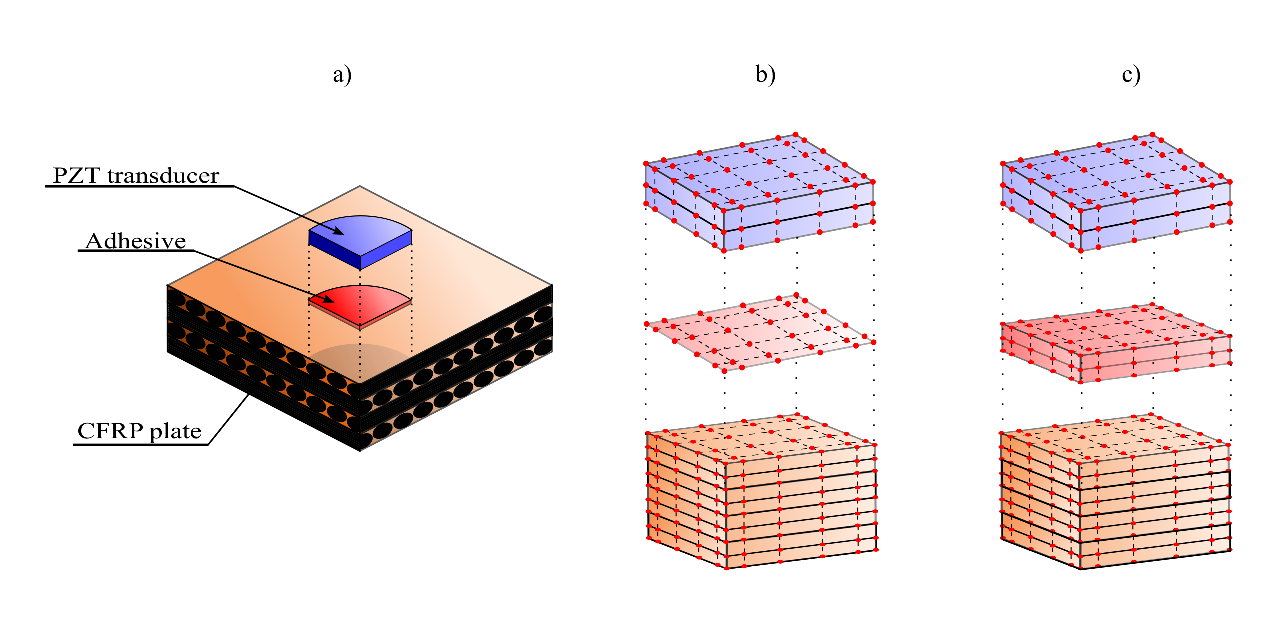
\includegraphics[width=1\textwidth]{Figures/structure.eps}
	\caption{Components used in the simulations. a)~Decomposition of components, b)~Spectral elements for the 2D-3D formulation, c)~Spectral elements for full 3D formulation}
	\label{fig:structure}
	\end{figure}
	
	\begin{table}
	\caption{Material properties of carbon fibres, epoxy resin and adhesive layer}
	\begin{tabular}{lccc} \hline
	Material & Young modulus [GPa] & Poisson's ratio [-] & Density [kg/m$^3$]\\ \hline
	Carbon & 275.6 & 0.2 & 1900\\
	Epoxy & 3.43 & 0.35 & 1250\\
	Adhesive & 3.0 & 0.34 & 1200\\ \hline
	\end{tabular}
	\label{tab:properties}
	\end{table}
	
	\subsection{50 kHz excitation results}
	For the excitation 50 kHz, a mesh with $931\:181$ Global Degrees of Freedom (GDoF) was generated. Fig. \ref{fig:wave_field} presents snapshots of the simulated and measured guided waves at the three different time intervals. As~it could be expected, the shape of propagating waves in the composite is not circular as in case of waves propagated in isotropic materials. Waves propagate faster at $0^o$ and $90^o$, when corresponds to the reinforcing fibres directions. Additionally, in the experimental signals reflections from delamination are visible at 289 $\mu s$. Delamination was not modelled in the current analysis.
	\begin{figure}
	\includegraphics[width=1\textwidth]{Figures/wave_field_snapshot.eps}
	\caption{Comparison between simulated and measured of full wavefield of the elastic wave propagated in CFRP plate for 50 kHz.}
	\label{fig:wave_field}
	\end{figure}
	
	Fig. \ref{fig:particle_V_50kHz} presents a plot of measured and simulated envelope of out--of--plane particle velocity signal in the two points $P_1=(60.2,\ 0^o)$ [mm, deg] and $P_2=(58.5,\ 45^o)$ [mm, deg]. One can see a distinct $A_0$ mode on the plot, while the $S_0$ mode is invisible because its amplitude is a few orders of magnitude less than the $A_0$ mode. The simulations results correlate excellently with the experimental data for both directions of propagated wave $0^o$ and $45^o$. The group velocity $(c_g)$ for the $A_0$ mode obtained in the simulation is only $3.8\%$ less than velocity measured experimentally (see Fig. \ref{fig:C_g}). The group velocity is calculated as follow:
	\begin{eqnarray}
	c_g=\frac{P_1-P_0}{TOF_1-TOF_0}
	\end{eqnarray}
	where $P_0$ and $P_1$ are coordinates of two points, $TOF_0$ and $TOF_1$ are time--of--flight of wave package to $P_0$ and $P_1$, respectively (see Fig. \ref{fig:TOF_50kHz}).
	\begin{figure}
	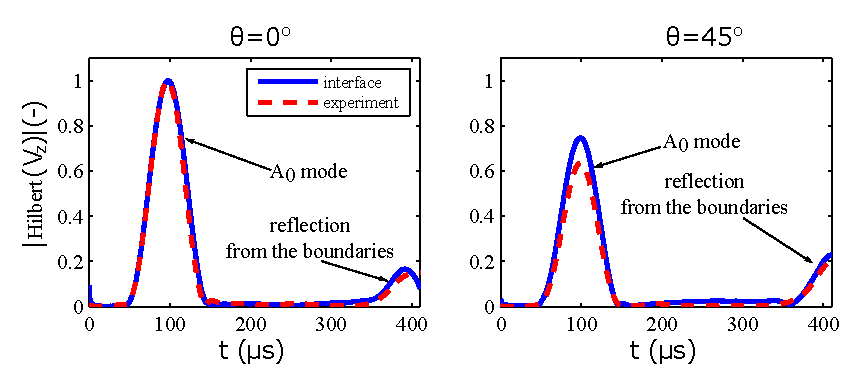
\includegraphics[width=1\textwidth]{Figures/50kHz.eps}
	\caption{Envelope of the out--of--plane particle velocity measured (dashed line) and calculated (solid line) at 60.2 mm distance from the centre and an angle direction $\theta=0^o$ for excitation frequency 50 kHz.}
	\label{fig:particle_V_50kHz}
	\end{figure}
	\begin{figure}
	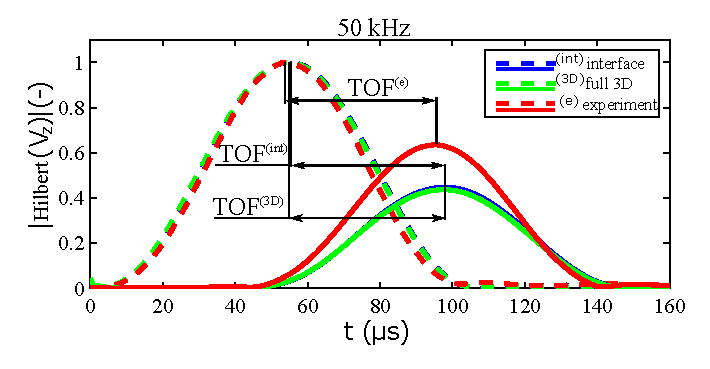
\includegraphics[width=1\textwidth]{Figures/TOF50kHz.eps}
	\caption{Time--of--flight (TOF) estimation. Envelope of out--of--plane velocity signal captured in point $P_0(5.3,\ 0^o)$ [mm, deg] (dashed line) and in point $P_1(60.2,\ 0^o)$ [mm, deg] (solid line) for excitation frequency 50 kHz.}
	\label{fig:TOF_50kHz}
	\end{figure}
	\begin{figure}
	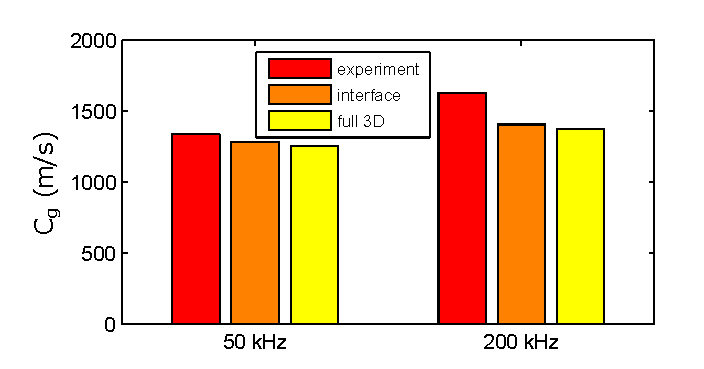
\includegraphics[width=1\textwidth]{Figures/C_g.eps}
	\caption{Comparison of the group velocity for $A_0$ mode for excitation frequency 50 kHz and 200 kHz.}
	\label{fig:C_g}
	\end{figure}
	\subsection{200 kHz excitation results}
	In the case of 200 kHz excitation, the fine mesh was generated, and the number of in--plane nodes was increased to 81 so that GDoF was $7\:034\:873$. Both modes $S_0$ (the first wavepacket) and $A_0$ (the second wavepacket) are noticeable in Fig. \ref{fig:particle_V_200kHz}. The simulation results are in good agreement with experimental data. However, the results of the $A_0$ mode are not as good as results of $S_0$. As it can be seen in Fig. \ref{fig:C_g}, the difference between the experimentally measured and numerically obtained value of the $c_g$ increased to $13.8\%$. The discrepancies may arise due to more complex, the antisymmetric character of displacements field, and shorter wavelength than $S_0$ mode. 
	
	\begin{figure}
	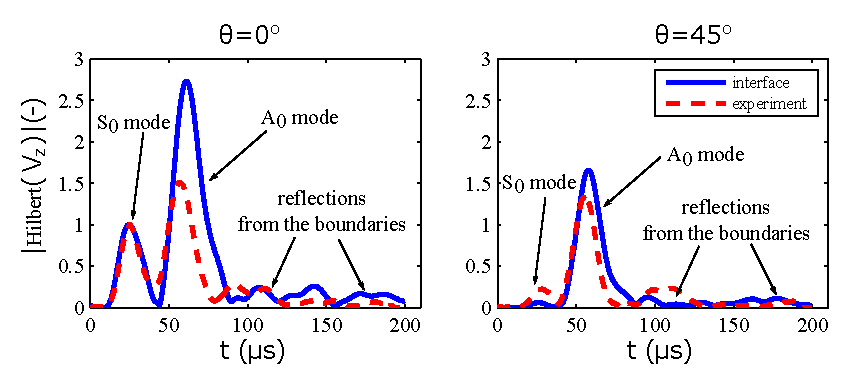
\includegraphics[width=1\textwidth]{Figures/200kHz.eps}
	\caption{Magnitude of the out--of--plane particle velocity measured (dashed line) and calculated (solid line) at 60.12 mm distance from the centre and an angle direction $\theta=0^o$ for 200 kHz excitation.}
	\label{fig:particle_V_200kHz}
	\end{figure}
	
	\subsection{Simulation of an adhesive thickness effect on guided waves}
	The present model of wave propagation in the composite plate was used for simulation of an adhesive thickness effect on GW. An amplitude of out--of--plane particle velocity was calculated concerning adhesive thickness for different excitation frequency. The simulation was made for a) adhesive thickness $h=(0,\ 50,\ 100)$~$\mu m$, and b) excitation frequency $f=(50,\ 100,\ 150,\ 200)$~kHz. 
	
	From the Fig. \ref{fig:Amp}, it can be noticed that the amplitude of $A_0$ mode decreases if the adhesive thickness increases. However, the influence of the adhesive thickness on this mode decreases with the increase of the excitation frequency. Excluding the case for the 150 kHz frequency, in which the amplitude is nearly reduced to zero.
	
	Conversely, in the case of $S_0$ mode, the amplitude increases with the increase of the adhesive thickness, and the differences are greater for higher excitation frequency. 
	\begin{figure}
	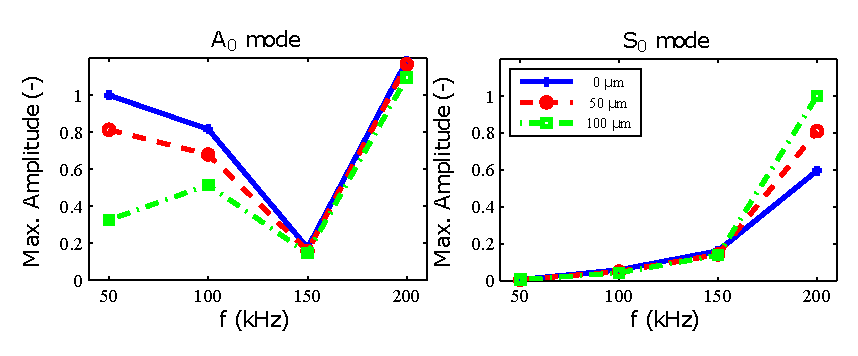
\includegraphics[width=1\textwidth]{Figures/Amp.eps}
	\caption{Normalized amplitude of out--of--plane particle velocity calculated in point $(60.12,\ 0^o)$ [mm, deg].}
	\label{fig:Amp}
	\end{figure}
	\subsection{2D vs 3D elements for modelling of the adhesive layer}
	The signals from simulation with the use of the interface for modelling of the adhesive layer are compared with the results obtained by using 3D elements for the entire mesh. The mesh for 3D model remains the same in--plane directions as the 2D model and has three nodes in the thickness direction. Comparison of two models is presented in Fig.~\ref{fig:2D_3D}. It can be noticed, the $S_0$ mode of the present model is in good agreement with the full 3D formulation. However, some discrepancies in phase velocity and signal amplitudes appear for the $A_0$ mode. The differences are more prominent with increasing the excitation frequency, and they arise due to more complex displacement field in the thickness direction of the $A_0$ than the $S_0$ mode. Applying a higher order plate theory can improve the accuracy of the solution.
	
	In order to compare both models according to time efficiency, a maximal time increment necessary for convergence of the equation of motion (\ref{eq:motion}) was estimated. It can be noticed from the Fig. \ref{fig:time_conver}a), that a value of displacement of the plate reaches infinity in after a certain number of time steps. In the case of 50 $\mu m$ of the adhesive layer thickness and 50 kHz excitation, maximal displacement reached the plate thickness after 405 time steps, \textit{i.e.} 4.67 $\mu s$ and monotonically rises to infinity. A convergence in SEM depends strictly on the distance between nodes of the used elements. Whereas the present model of the adhesive layer has only one node through the thickness $\Delta t$ depends on the smallest element of the remaining components (\textit{i.e.} CFRP plate and PZT). In case of the 3D model, the time increment is equal to $\Delta t_0=0.01154\ \mu s$ (minimal time increment for non--adhesive layer model) for the adhesive thickness over 40 $\mu m$, the significant decreasing of the $\Delta t$ is observed in the range 1--20 $\mu m$ as it is shown on the Fig. \ref{fig:time_conver}b).
	\begin{figure}
	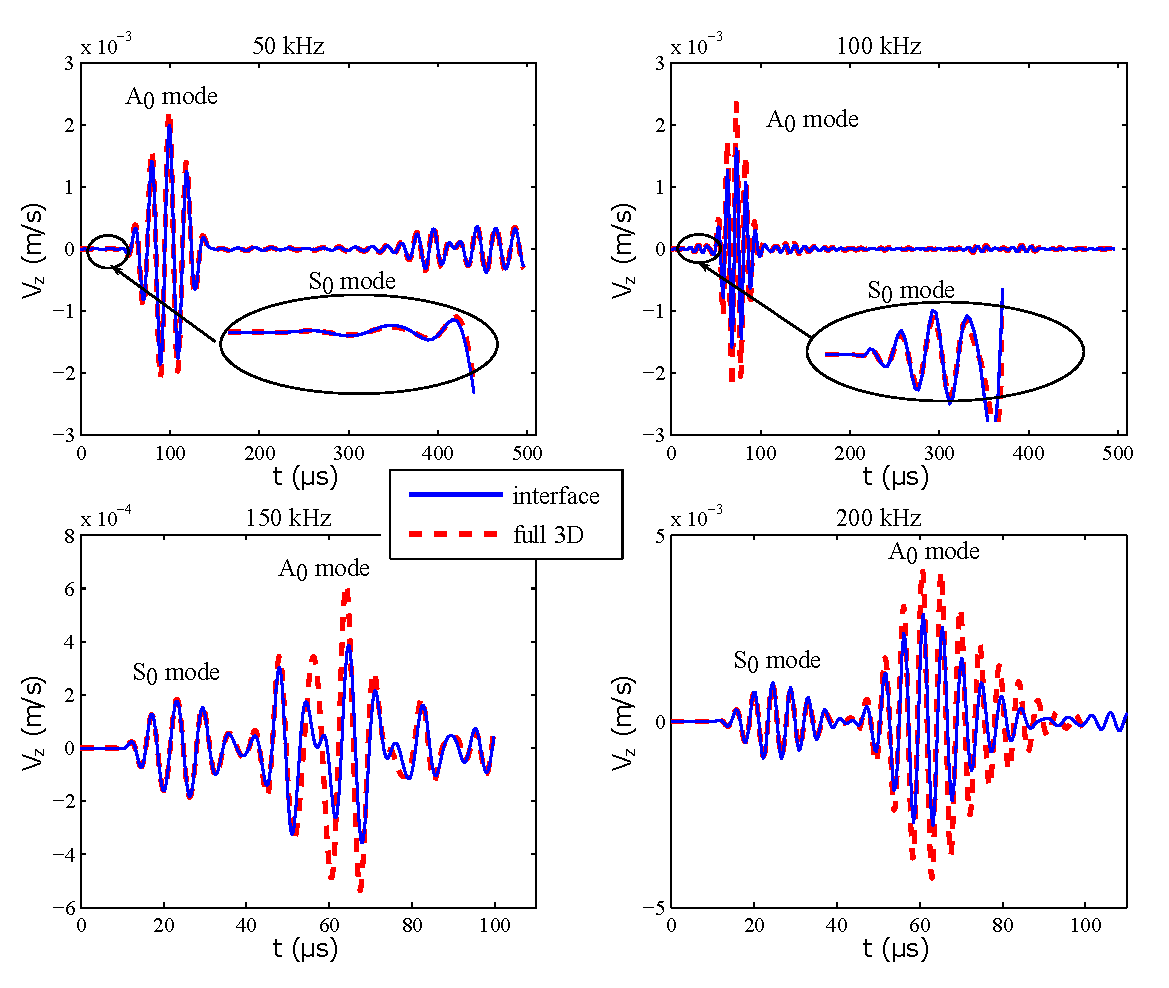
\includegraphics[width=1\textwidth]{Figures/2D_3D.eps}
	\caption{Simulated signals of out--of--plane particle velocity at the point $(60.12,\ 0^o)$ [mm, deg] in case of 3D (dashed line), and 2D (solid line) model of the adhesive layer.} 
	\label{fig:2D_3D}
	\end{figure}
	\begin{figure}
	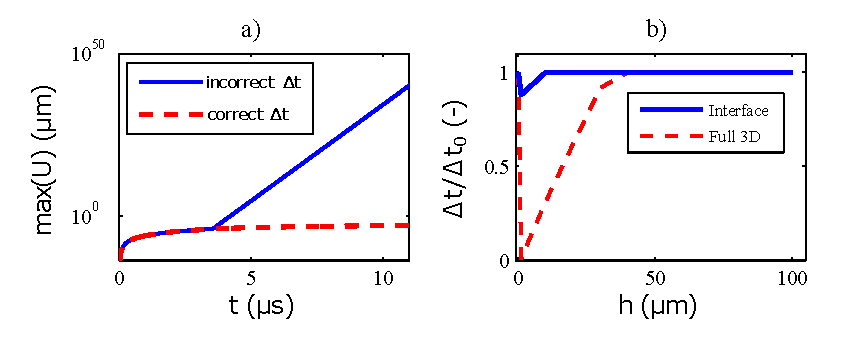
\includegraphics[width=1\textwidth]{Figures/time_conver.eps}
	\caption{Convergence of the time integration equation for 50 $\mu m$ of adhesive layer and 50 kHz excitation. a) Maximal displacement of the top surface of the plate for incorrect (solid line) and correct (dashed line) chosen time step; b) minimal correct time step for 3D (dashed line) and 2D (solid line) elements, normalized to $\Delta t_0$.}
	\label{fig:time_conver}
	\end{figure}
	
	\section{Conclusions}
	In this paper, a new approach for spectral finite element formulation has been successfully developed. Lagrange multipliers were used to impose the displacements coupling between 2D and 3D spectral elements for the numerical simulation of elastic wave propagation in a composite material. Results obtained in the simulations are in good agreement with experimental measurements. The present model was used for simulation an effect of the adhesive layer thickness on guided waves propagation. This model significantly decreases the computation time, while a required number of time steps is from 47600 to 1.6 times fewer in comparison to full 3D model in the range of thickness dimension from 1 to 20 $\mu m$, respectively, for assumed total simulation time $T_s=500$ $\mu s$. 
	
	This approach assumed matching grids in the interface between two substructures so in the next step for more flexibility the non--matching grids will be introduced.
	\end{comment}
	%% The Appendices part is started with the command \appendix;
	%% appendix sections are then done as normal sections
	%% \appendix
	%% \section{}
	%% \label{}
	\section*{Acknowledgement}
	The research was funded by the Polish National Science Center under grant agreement no 
	
	
	
	%% If you have bibdatabase file and want bibtex to generate the
	%% bibitems, please use
	%%
	%%  \bibliographystyle{elsarticle-harv} 
	%%  \bibliography{<your bibdatabase>}
	
	%% else use the following coding to input the bibitems directly in the
	%% TeX file.
	\section*{Reference}
	\bibliography{BibTeX_interface}{}
	\bibliographystyle{num_order}
\end{document}


